\section{内存架构和数据局部性}
到目前为止,我们已经学习了如何编写 CUDA kernel函数以及如何配置和协调大量线程的执行。 
我们还研究了当前 GPU 硬件的计算架构以及如何调度线程在该硬件上执行。 
在本章中,我们将重点关注on-chip的内存架构,并开始研究如何组织和定位数据,以便大量线程进行高效访问。 
到目前为止,我们研究的 CUDA kernel可能只能发挥出底层硬件性能的一小部分。 
这种糟糕的性能是因为通常使用off-chip内存实现的全局内存往往具有较长的访问延迟(数百个时钟周期)和有限的访问带宽。 
虽然拥有许多可供执行的线程理论上可以容忍较长的内存访问延迟,
人们很容易遇到这样一种情况:全局内存访问路径中的流量拥塞导致除极少数线程之外的所有线程都无法取得进展,
从而导致流式多处理器 (SM) 中的某些核心处于空闲状态。 为了避免这种拥塞,GPU 提供了许多额外的on-chip内存资源来访问数据,
从而消除了进出全局内存的大部分流量。 在本章中,我们将研究如何使用不同的内存类型来提高 CUDA kernel的执行性能。

\subsection{内存访问效率的重要性}
\begin{figure}[H]
	\centering
	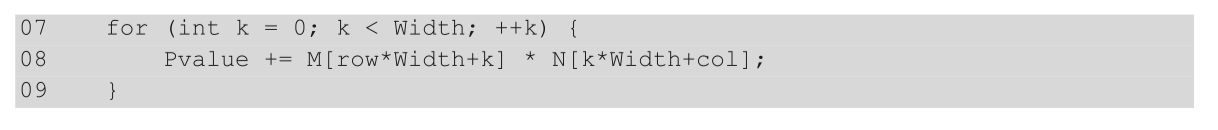
\includegraphics[width=0.9\textwidth]{figs/F5.1.png}
	\caption{\textit{图 3.11 中矩阵乘法kernel执行最多的部分。}}
\end{figure}

我们可以通过计算图 3.11 中矩阵乘法kernel代码执行最多的部分的预期性能水平来说明内存访问效率的影响,
该部分在图 5.1 中进行了部分复制。 就执行时间而言,kernel最重要的部分是 for 循环,它执行 M 行与 N 列的点积。

在循环的每次迭代中,针对一次浮点乘法和一次浮点加法执行两次全局内存访问。 全局内存访问从 M 和 N 数组中获取元素。 
浮点乘法运算将这两个元素相乘,浮点加法运算将乘积累加到 Pvalue 中。 
因此,浮点运算 (FLOP) 与从全局内存访问的字节 (B) 的比率为 2 FLOP 比 8 B,即 0.25 FLOP/B。 
我们将此比率称为计算与全局内存访问比率,定义为程序某个区域内从全局内存访问每个字节所执行的 FLOP 次数。 
在文献中,该比率有时也称为算术强度或计算强度。

计算与全局内存访问的比率对 CUDA kernel的性能有重大影响。 例如,Ampere A100 GPU 的峰值全局内存带宽为 1555 GB/秒。 
由于矩阵乘法kernel执行 0.25 OP/B,因此全局内存带宽将kernel可执行的单精度 FLOP 的吞吐量限制为每秒 389 GB FLOP(GFLOPS),
这是通过将 1555 GB/秒乘以 0.25 FLOP 获得的 /B。 
然而,389 GFLOPS 仅为 A100 GPU 峰值单精度运算吞吐量(19,500 GFLOPS)的 2\%。 
A100 还配备了称为张量核心的特殊用途单元,可用于加速矩阵乘法运算。 
如果考虑 A100 的张量核心峰值单精度浮点吞吐量为 156,000 GFLOPS,则 389 GFLOPS 仅是峰值的 0.25\%。 
因此,矩阵乘法kernel的执行受到数据从内存传送到 GPU kernel的速率的严重限制。 
我们将执行速度受内存带宽限制的程序称为内存限制程序。

为了使该kernel获得更高的性能,我们需要通过减少kernel执行的全局内存访问次数来提高kernel的计算与全局内存访问的比率。 
例如,要充分利用A100 GPU提供的19,500 GFLOPS,至少需要(19,500 GOP/秒)/(1555 GB/秒)=12.5 OP/B的比率。 
这个比率意味着每访问一个 4 字节浮点值,必须执行大约 50 次浮点运算! 
能够实现这一比率的程度取决于当前计算中的内在数据重用。 我们建议读者参考“Roofline 模型”侧边栏,
了解一个有用的模型,用于分析程序相对于计算强度的潜在性能。

正如我们将看到的,矩阵乘法提供了减少全局内存访问的机会,这可以通过相对简单的技术来捕获。 
矩阵乘法函数的执行速度可能会变化几个数量级,具体取决于全局内存访问的减少程度。 
因此,矩阵乘法为此类技术提供了一个很好的初始示例。 本章介绍了一种减少全局内存访问次数的常用技术,并演示了矩阵乘法技术。

\begin{remark}[Roofline 模型]
Roofline 模型是一种可视化模型,用于评估应用程序相对于其运行的硬件限制所实现的性能。 
Roofline 模型的基本示例如下所示。

\begin{figure}[H]
	\centering
	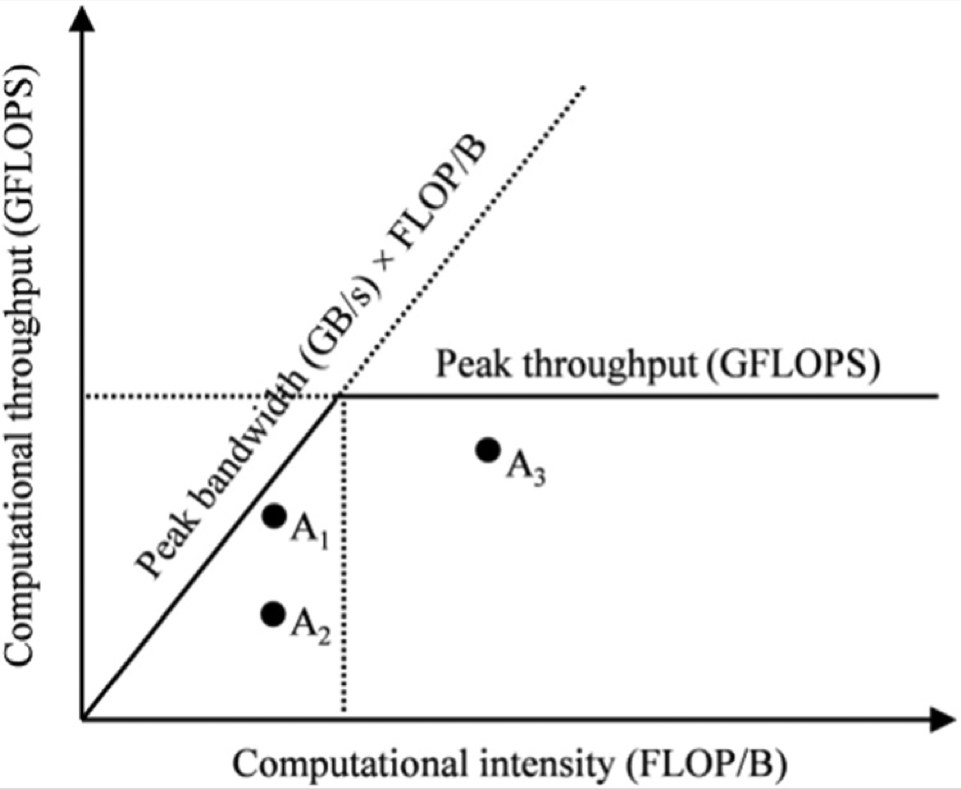
\includegraphics[width=0.9\textwidth]{figs/F5-a.1.png}
\end{figure}

在 x 轴上,我们以 FLOP/B 为单位测量算术或计算强度。 它反映了应用程序为加载的每个字节数据完成的工作量。 
在 y 轴上,我们以 GFLOPS 为单位测量计算吞吐量。 图中的两条线反映了硬件限制。 
水平线由硬件可以承受的峰值计算吞吐量 (GFLOPS) 决定。 从原点开始的正斜率线由硬件可以承受的峰值内存带宽决定。 
图中的点代表应用程序,其运行强度在 x 轴上,其实现的计算吞吐量在 y 轴上。 
当然,这些点将位于两条线下方,因为它们无法实现比硬件峰值更高的吞吐量。

点相对于两条线的位置告诉我们应用程序的效率。 靠近两条线的点表示应用程序正在有效地使用内存带宽或计算单元,
而远低于两条线的应用程序表示资源使用效率低下。 两条线之间的交点表示应用程序从内存限制转变为计算限制时的计算强度值。 
计算强度较低的应用程序受内存限制,无法实现峰值吞吐量,因为它们受到内存带宽的限制。 
计算强度较高的应用程序受计算限制,并且不受内存带宽的限制。

例如,点 $A_1$ 和 $A_2$ 都表示内存限制型应用程序,而 $A_3$ 表示计算限制型应用程序。 
$A_1$ 有效地使用资源并在接近峰值内存带宽的情况下运行,而 $A_2$ 则不然。 
对于 $A_2$,可能存在额外优化的空间,以通过提高内存带宽利用率来提高吞吐量。 
然而,对于 $A_1$ 来说,提高吞吐量的唯一方法是增加应用程序的计算强度。
\end{remark}

\subsection{CUDA 内存类型}
\begin{figure}[H]
	\centering
	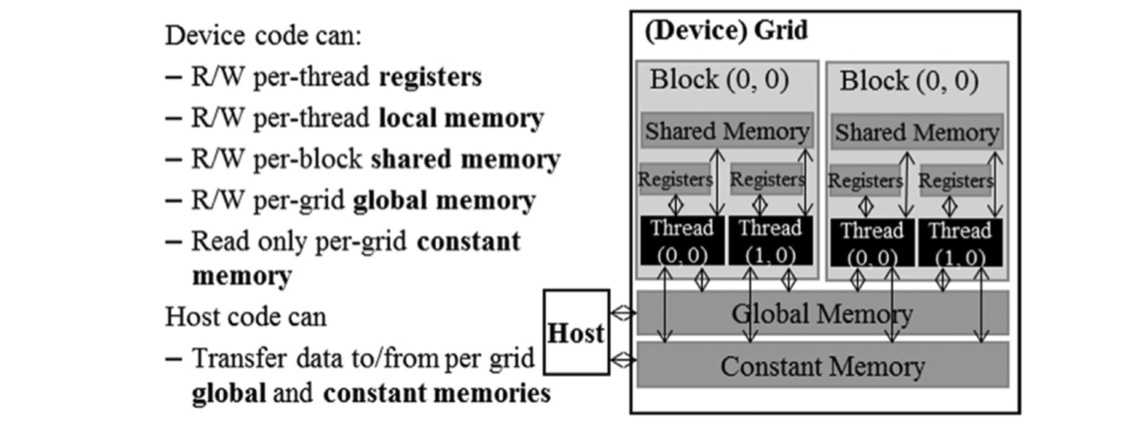
\includegraphics[width=0.9\textwidth]{figs/F5.2.png}
	\caption{\textit{CUDA GPU内存模型的(不完整)概述。 
	图中未显示的一种重要类型的 CUDA 内存是纹理内存,因为本教科书未介绍其使用。}}
\end{figure}

CUDA GPU包含多种类型的内存,可以帮助程序员提高计算与全局内存访问的比率。 图 5.2 显示了这些 CUDA GPU内存。 
在图的底部,我们看到全局内存和常量内存。 这两种类型的内存都可以由CPU写入(W)和读取(R)。 
全局内存也可以由GPU写入和读取,而常量内存支持GPU的短延迟、高带宽只读访问。 
我们在第 2 章“异构数据并行计算”中介绍了全局内存,我们将在第 7 章“卷积”中详细介绍常量内存。

另一种类型的内存是本地内存,它也可以读写。 本地内存实际上放置在全局内存中,并且具有类似的访问延迟,但它不跨线程共享。 
每个线程都有自己的全局内存部分,将其用作自己的私有本地内存,其中放置线程私有但无法在寄存器中分配的数据。 
这些数据包括静态分配的数组、溢出的寄存器和线程调用堆栈的其他元素。

图5.2中的寄存器和共享内存是on-chip内存。 可以以高度并行的方式以非常高的速度访问驻留在这些类型的内存中的变量。 
寄存器被分配给各个线程; 每个线程只能访问自己的寄存器(请参阅“CPU 与 GPU 寄存器架构”边栏)。 
kernel函数通常使用寄存器来保存每个线程私有的频繁访问的变量。 共享内存分配给线程块; 
块中的所有线程都可以访问为该块声明的共享内存变量。 共享内存是一种有效的方式,
线程可以通过共享它们的输入数据和中间结果来进行协作。 通过在一种 CUDA 内存类型中声明 CUDA 变量,
CUDA 程序员可以规定该变量的可见性和访问速度。

\begin{remark}[CPU 与 GPU 寄存器架构]
CPU 和 GPU 的不同设计目标导致不同的寄存器架构。 正如我们在第 4 章“计算架构和调度”中看到的,
当 CPU 在不同线程之间进行上下文切换时,它们会将传出线程的寄存器保存到内存中,并从内存中恢复传入线程的寄存器。 
相比之下,GPU 通过将处理块上调度的所有线程的寄存器保留在处理块的寄存器文件中来实现零开销调度。 
这样,线程线程束之间的切换是瞬时的,因为传入线程的寄存器已经在寄存器文件中。 
因此,GPU 寄存器文件需要比 CPU 寄存器文件大得多。

我们还在第 4 章“计算架构和调度”中看到,GPU 支持动态资源分区,其中 SM 可以为每个线程提供少量寄存器并执行大量线程,
或者为每个线程提供更多寄存器并执行更少线程。 因此,GPU 寄存器文件需要设计为支持寄存器的动态分区。 
相比之下,CPU 寄存器架构为每个线程专用一组固定的寄存器,而不管线程对寄存器的实际需求如何。
\end{remark}

\begin{figure}[H]
	\centering
	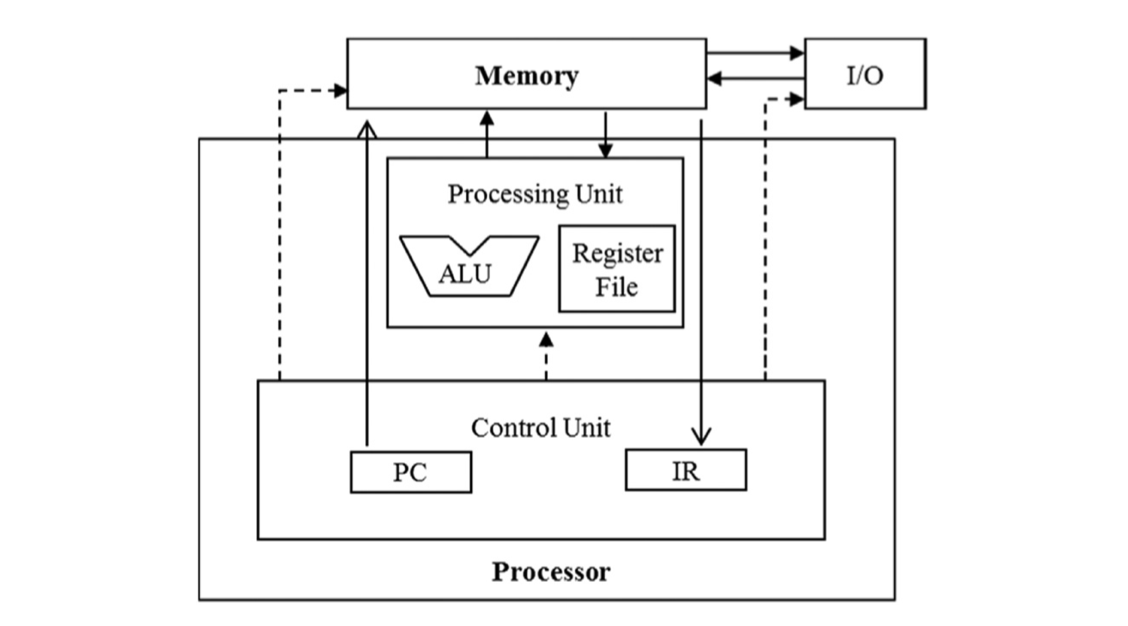
\includegraphics[width=0.9\textwidth]{figs/F5.3.png}
	\caption{\textit{基于冯·诺依曼模型的现代计算机中的内存与寄存器。}}
\end{figure}

为了充分理解寄存器、共享内存和全局内存之间的区别,我们需要更详细地了解这些不同的内存类型在现代处理器中是如何实现和使用的。 
正如我们在第 4 章“计算架构和调度”的“Warps 和 SIMD 硬件”边栏中讨论的那样,
几乎所有现代处理器都源于 John von Neumann 在 1945 年提出的模型,如图 5.3 所示。 
CUDA GPU也不例外。 CUDA GPU中的全局内存映射到图 5.3 中的内存框。 
处理器区域对应于我们今天通常看到的处理器芯片边界。 全局内存脱离处理器芯片并采用 DRAM 技术实现,
这意味着较长的访问延迟和相对较低的访问带宽。 寄存器对应于冯·诺依曼模型的“寄存器文件”。 
寄存器文件位于处理器芯片上,这意味着与全局内存相比,访问延迟非常短,并且访问带宽显着提高。 
在典型的GPU中,所有 SM 上的所有寄存器文件的聚合访问带宽至少比全局内存高两个数量级。 
此外,每当变量存储在寄存器中时,其访问不再消耗off-chip全局内存带宽。 这将反映为计算与全局内存访问比率的增加。

更微妙的一点是,每次对寄存器的访问所涉及的指令比对全局内存的访问要少。 
大多数现代处理器中的算术指令都有“内置”寄存器操作数。 例如,浮点加法指令可能具有以下形式:

fadd r1, r2, r3

其中 r2 和 r3 是寄存器编号,指定寄存器文件中可以找到输入操作数值的位置。 
浮点加法结果值的存储位置由r1指定。 因此,当算术指令的操作数位于寄存器中时,
不需要额外的指令来使操作数值可用于完成算术计算的算术和逻辑单元(ALU)。

同时,如果操作数值位于全局内存中,则处理器需要执行内存加载操作以使操作数值可供ALU使用。 
例如,如果浮点加法指令的第一个操作数位于全局内存中,则所涉及的指令可能类似于以下示例:

load r2, r4, offset

fadd r1, r2, r3

其中加载指令将偏移值添加到 r4 的内容以形成操作数值的地址。 然后它访问全局内存并将值放入寄存器 r2 中。 
一旦操作数值位于 r2 中,fadd 指令就会使用 r2 和 r3 中的值执行浮点加法,并将结果放入 r1 中。 
由于处理器每个时钟周期只能获取和执行有限数量的指令,因此具有额外负载的版本可能会比没有负载的版本花费更多的时间来处理。 
这也是为什么将操作数放在寄存器中可以提高执行速度的另一个原因。

最后,还有另一个微妙的原因为什么最好将操作数值放入寄存器中。 
在现代计算机中,从寄存器堆访问值所消耗的能量比从全局内存访问值所消耗的能量至少低一个数量级。 
与从全局内存访问值相比,从寄存器访问值在能源效率方面具有巨大优势。 
我们很快就会了解现代计算机中访问这两种硬件结构的速度和能量差异的更多细节。 
另一方面,我们很快就会了解到,在当今的 GPU 中,每个线程可用的寄存器数量非常有限。 
正如我们在第 4 章“计算架构和调度”中看到的,如果满占用场景中的寄存器使用量超过限制,则应用程序实现的占用率可能会减少。 
因此,我们还需要尽可能避免过度调度这一有限的资源。

\begin{figure}[H]
	\centering
	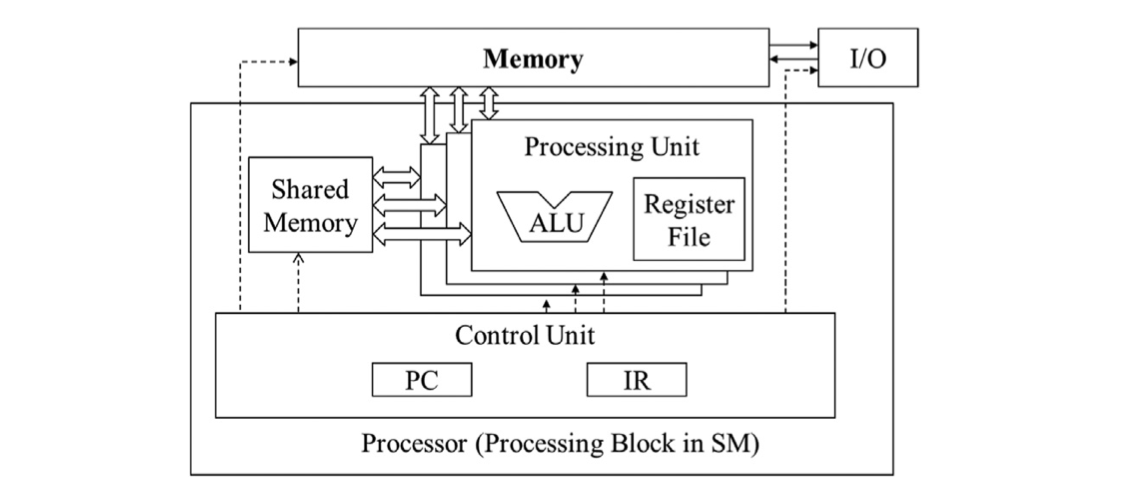
\includegraphics[width=0.9\textwidth]{figs/F5.4.png}
	\caption{\textit{CUDA GPU SM 中的共享内存与寄存器。}}
\end{figure}

图 5.4 显示了 CUDA GPU中的共享内存和寄存器。 尽管两者都是on-chip内存,但它们在功能和访问成本方面存在显着差异。 
共享内存被设计为驻留在处理器芯on-chip的内存空间的一部分。 
当处理器访问驻留在共享内存中的数据时,它需要执行内存加载操作,就像访问全局内存中的数据一样。 
然而,由于共享内存驻留在on-chip,因此与全局内存相比,它的访问延迟要低得多,吞吐量要高得多。 
由于需要执行加载操作,共享内存比寄存器具有更长的延迟和更低的带宽。 
在计算机体系结构术语中,共享内存是暂存器内存的一种形式。

CUDA 中的共享内存和寄存器之间的一个重要区别是,驻留在共享内存中的变量可由块中的所有线程访问。 
这与寄存器数据形成对比,寄存器数据是线程私有的。 也就是说,共享内存旨在支持块中线程之间高效、高带宽的数据共享。 
如图 5.4 所示,CUDA GPU SM 通常采用多个处理单元来允许多个线程同时进行(参见第 2 章异构数据并行计算中的“线程”侧边栏)。 
块中的线程可以分布在这些处理单元上。 
因此,这些 CUDA GPU中共享内存的硬件实现通常被设计为允许多个处理单元同时访问其内容,以支持块中线程之间的高效数据共享。 
我们将学习几种重要类型的并行算法,这些算法可以从线程之间有效的数据共享中受益匪浅。

\begin{table}[H]
\centering
\begin{tabular}{l|l|l|l}
	Variable declaration & Memory & Scope & Lifetime \\
	Automatic variables other than arrays & Register & Thread & Grid \\
	Automatic array variables & Local & Thread & Grid \\
	\_\_device\_\_ \_\_shared\_\_ int SharedVar; & Shared & Block & Grid \\
	\_\_device\_\_ int GlobalVar; & Global & Grid & Application \\
	\_\_device\_\_ \_\_constant\_\_ int ConstVar; & Constant & Grid & Application \\
\hline
\end{tabular}
\caption{CUDA 变量声明类型限定符和每种类型的属性。}
\end{table}

现在应该清楚了,寄存器、本地内存、共享内存和全局内存都具有不同的功能、延迟和带宽。 
因此,了解如何声明变量以使其驻留在预期类型的内存中非常重要。 表 5.1 介绍了将程序变量声明到各种内存类型中的 CUDA 语法。 
每个这样的声明还为其声明的 CUDA 变量提供了范围和生命周期。 
作用域标识了可以访问变量的线程集:仅限单个线程,grid的所有线程或所有grid的所有线程。 
如果变量的作用域是单线程,则将为每个线程创建该变量的私有版本; 每个线程只能访问该变量的私有版本。 
例如,如果kernel声明了一个作用域为线程的变量,并且使用一百万个线程启动该变量,
则将创建该变量的一百万个版本,以便每个线程初始化并使用自己的变量版本。

生命周期告诉变量可供使用时程序执行持续时间的一部分:无论是在grid执行中还是在整个应用程序中。 
如果变量的生命周期在grid执行期间,则必须在kernel函数体内声明它,并且只能由kernel代码使用。 
如果多次调用kernel,则在这些调用中不会维护该变量的值。 每次调用都必须初始化变量才能使用它。 
另一方面,如果变量的生命周期贯穿整个应用程序,则必须在任何函数体之外声明它。 
这些变量的内容在应用程序的整个执行过程中得到维护,并且可供所有kernel使用。

我们将非数组的变量称为标量变量。 如表 5.1 所示,在kernel和GPU函数中声明的所有自动标量变量都放入寄存器中。 
这些自动变量的范围在各个线程内。 当kernel函数声明自动变量时,将为执行该kernel函数的每个线程生成该变量的私有副本。 
当线程终止时,它的所有自动变量都不再存在。 
在图5.1中,变量blurRow、blurCol、curRow、curCol、pixels和pixVal都是自动变量,属于这一类。 
请注意,访问这些变量的速度非常快并且是并行的,但必须小心不要超出硬件实现中寄存器存储的有限容量。 
使用大量寄存器会对每个 SM 的占用产生负面影响,正如我们在第 4 章“计算架构和调度”中看到的那样。

自动数组变量不存储在寄存器中
\footnote{此规则有一些例外。 如果所有访问都是使用常量索引值完成的,则编译器可能会决定将自动数组存储到寄存器中。} 。
相反,它们存储在线程的本地内存中,可能会导致较长的访问延迟和潜在的访问拥塞。 
这些数组的范围与自动标量变量的范围一样,仅限于单个线程。 也就是说,为每个线程创建并使用每个自动数组的私有版本。 
一旦线程终止执行,其自动数组变量的内容就不再存在。 根据我们的经验,在kernel函数和GPU函数中很少需要使用自动数组变量。

如果变量声明前面有 \_\_shared\_\_ 关键字(每个“\_\_”由两个“\_”字符组成),则在 CUDA 中声明一个共享变量。 
还可以在声明中的 \_\_shared\_\_ 前面添加一个可选的 \_\_device\_\_ 来达到相同的效果。 
这种声明通常在kernel函数或GPU函数中进行。 共享变量驻留在共享内存中。 共享变量的作用域是在一个线程块内; 
也就是说,块中的所有线程都看到共享变量的相同版本。 在kernel执行期间,为每个块创建并使用共享变量的私有版本。 
共享变量的生存期在kernel执行的持续时间内。 当kernel终止其grid的执行时,其共享变量的内容将不再存在。 
正如我们之前讨论的,共享变量是块内线程相互协作的有效手段。 从共享内存访问共享变量非常快并且高度并行。 
CUDA 程序员经常使用共享变量来保存在kernel执行阶段频繁使用和重用的全局内存数据部分。 
人们可能需要调整用于创建主要关注全局内存数据的一小部分的执行阶段的算法,
正如我们将在第 5.4 节中通过矩阵乘法进行演示的那样。

如果变量声明前面有关键字 \_\_constant\_\_'(每个“\_\_”由两个“\_”字符组成),则它在 CUDA 中声明一个常量变量。 
还可以在 \_\_constant\_\_ 前面添加一个可选的 \_\_device\_\_ 来达到相同的效果。 常量变量的声明必须在任何函数体之外。 
常量变量的作用域是所有grid,这意味着所有grid中的所有线程都看到相同版本的常量变量。 
常量变量的生命周期是整个应用程序执行的时间。 常量变量通常用于为核函数提供输入值的变量。 
常量变量的值不能由kernel函数代码更改。 常量变量存储在全局内存中,但会被缓存以便有效访问。 
通过适当的访问模式,访问常量内存的速度非常快并且是并行的。 目前,应用程序中常量变量的总大小限制为 65,536 字节。 
人们可能需要分解输入数据量以适应这一限制。 我们将在第 7 章“卷积”中演示常量内存的用法。

声明前面仅带有关键字 \_\_device\_\_ (每个“\_\_”由两个“\_”字符组成)的变量是全局变量,将被放置在全局内存中。 
对全局变量的访问速度很慢。 在较新的GPU中,通过缓存改进了访问全局变量的延迟和吞吐量。 
全局变量的一个重要优点是它们对所有kernel的所有线程都是可见的。 它们的内容也会在整个执行过程中持续存在。 
因此,全局变量可以用作线程跨块协作的手段。 然而,我们必须意识到,除了使用原子操作或终止当前kernel执行之外,
目前还没有一种简单的方法可以在不同线程块的线程之间进行同步,或者在访问全局内存时确保线程之间的数据一致性
\footnote{如果线程块的数量小于 CUDA GPU中 SM 的数量,则可以使用 CUDA 内存防护来确保线程块之间的数据一致性。 
有关详细信息,请参阅 CUDA 编程指南。}。 
因此,全局变量通常用于将信息从一个kernel调用传递到另一kernel调用。

在CUDA中,指针可以用来指向全局内存中的数据对象。 在kernel和GPU函数中,指针的使用有两种典型的方式。 
首先,如果一个对象是由CPU函数分配的,则指向该对象的指针将由内存分配API函数(例如cudaMalloc)初始化,
并且可以作为参数传递给kernel函数,正如我们在第2章异构数据并行计算中看到的那样 ,以及第 3 章,多维grid和数据。 
第二种用法是将全局内存中声明的变量的地址赋给指针变量。 
例如,kernel函数中的语句{float* ptr=\&GlobalVar;}将GlobalVar的地址赋给自动指针变量ptr。 
有关在其他内存类型中使用指针的信息,读者应参阅 CUDA 编程指南。

\subsection{tile(Tiling)以减少内存流量}
在 CUDA 中使用GPU内存时,我们有一个内在的权衡:全局内存大但速度慢,而共享内存小但速度快。 
常见的策略是将数据划分为称为tiles的子集,以便每个tile适合共享内存。 
术语“tile”比喻为大体积(即全局内存数据)可以被小tile(即可以放入共享内存的子集)覆盖。 
一个重要的标准是这些tile上的kernel计算可以彼此独立地完成。 请注意,在给定任意核函数的情况下,
并非所有数据结构都可以划分为tile。

\begin{figure}[H]
	\centering
	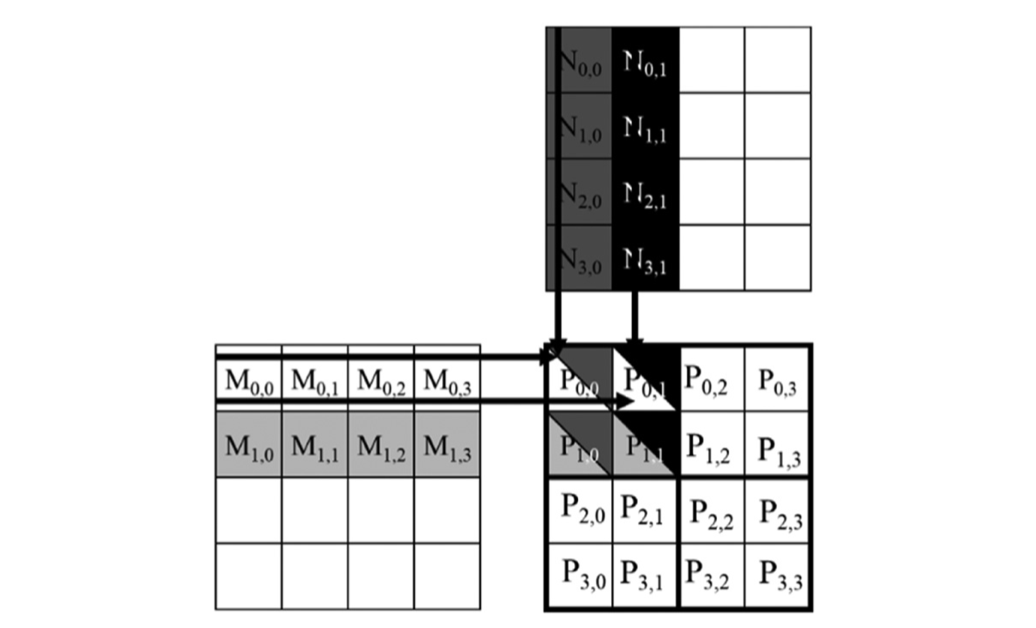
\includegraphics[width=0.9\textwidth]{figs/F5.5.png}
	\caption{\textit{矩阵乘法的一个小例子。 为了简洁起见,我们将 M[y * Width+x]、N[y * Width+x]、
	P[y * Width+x] 分别显示为 M\_{y,x} 、N\_{y,x} P\_{y,x}。}}
\end{figure}

tile的概念可以通过第 3 章“多维grid和数据”中的矩阵乘法示例来说明。 图 3.13 显示了矩阵乘法的一个小例子。 
它对应于图3.11中的核函数。 为了方便参考,我们复制图 5.5 中的示例。 
为了简洁起见,我们将 $P[y * Width+x]$、$M[y * Width+x]$ 和 $N[y * Width+x]$ 
分别缩写为 $P_{y,x}$ 、$M_{y, x}$ 和 $N_{y,x}$ 。 
此示例假设我们使用四个 $\times 2$ blocks来计算 P 矩阵。 P 矩阵中的粗框定义了每个block处理的 P 的元素。 
图 5.5 突出显示了 $block_{0,0}$ 的四个线程完成的计算。 
这四个线程计算 $P_{0,0}$ 、 $P_{0,1}$ 、 $P_{1,0}$ 和 $P_{1,1}$ 。 
$block_{0,0}$ 的 $thread_{0,0}$ 和 $thread_{0,1}$ 对 M 和 N 元素的访问用黑色箭头突出显示。 
例如,$thread_{0,0}$ 读取 $M_{0,0}$ 和 $N_{0,0}$ ,
接着依次为 $M_{0,1}$ 和 $N_{1,0}$ 、$M_{0,2}$ 和 $N_{2,0}$ 、$M_{0,3}$ 和 $N_{3,0}$ 。

\begin{figure}[H]
	\centering
	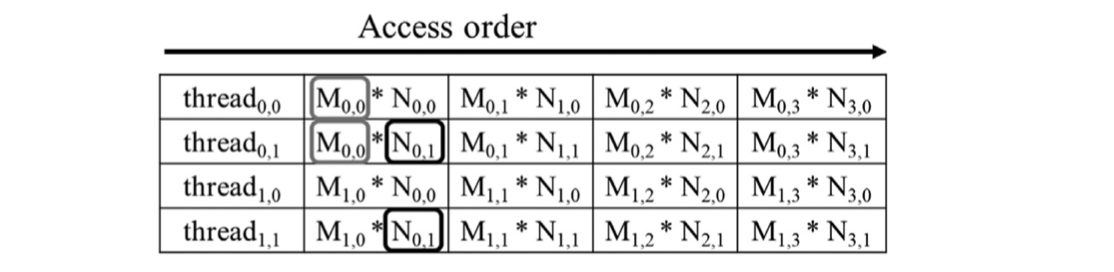
\includegraphics[width=0.9\textwidth]{figs/F5.6.png}
	\caption{\textit{由 $block_{0,0}$ 中的线程执行的全局内存访问。}}
\end{figure}

图 5.6 显示了 $block_{0,0}$ 中所有线程完成的全局内存访问。 线程按垂直方向列出,访问时间按水平方向从左到右递增。 
请注意,每个线程在执行期间都会访问 M 的四个元素和 N 的四个元素。 
在突出显示的四个线程中,它们访问的 M 和 N 元素存在显着重叠。 
例如,$thread_{0,0}$ 和 $thread_{0,1}$ 都访问 $M_{0,0}$ 以及 M 的第 0 行的其余部分。
类似地,$thread_{0,1}$ 和 $thread_{1,1}$ 都访问 $N_{0,1}$ 以及 N 的第 1 列的其余部分。

图 3.11 中的kernel被编写为 $thread_{0,0}$ 和 $thread_{0,1}$ 都从全局内存访问 M 的第 0 行元素。 
如果我们能够以某种方式设法让 $thread_{0,0}$ 和 $thread_{0,1}$ 协作,以便这些 M 元素仅从全局内存加载一次,
那么我们可以将对全局内存的访问总数减少一半。 事实上,我们可以看到,在 $block_{0,0}$ 的执行过程中,
每个 M 和 N 元素都被访问了两次。 因此,如果我们可以让所有四个线程协作访问全局内存,我们就可以将全局内存的流量减少一半。

读者应该验证矩阵乘法示例中访问全局内存潜在的减少空间与所使用的block的尺寸成正比。 
使用 Width $\times$ Width blocks,全局内存流量的潜在减少方向将是宽度。 
也就是说,如果我们使用 $16 \times 16$ 个 blocks,我们可以通过线程之间的协作将全局内存流量减少到原始水平的 1/16。

我们现在提出一种tile矩阵乘法算法。 基本思想是让线程协作将 M 和 N 元素的子集加载到共享内存中,
然后再在点积计算中单独使用这些元素。 请记住,共享内存的大小相当小,在将这 M 和 N 个元素加载到共享内存中时必须小心,
不要超过共享内存的容量。 这可以通过将 M 和 N 矩阵划分为更小的tile来实现。 
这些tile的大小经过选择,以便它们可以适合共享内存。 在最简单的形式中,tile的尺寸等于block的尺寸,如图 5.7 所示。

\begin{figure}[H]
	\centering
	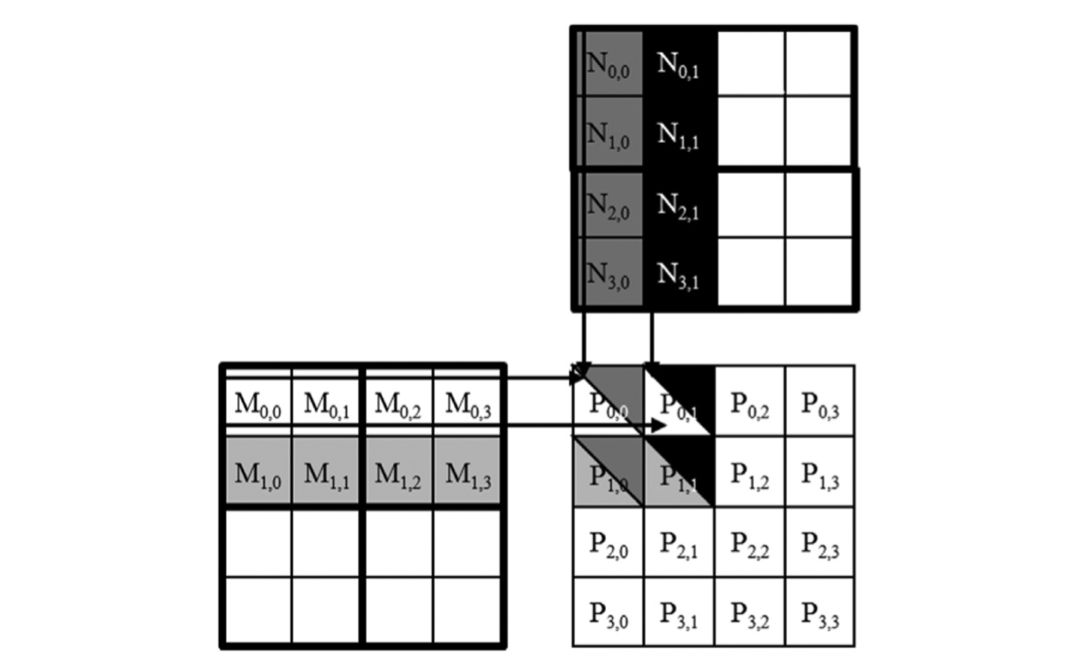
\includegraphics[width=0.9\textwidth]{figs/F5.7.png}
	\caption{\textit{tile M 和 N 以利用共享内存。}}
\end{figure}

在图 5.7 中,我们将 M 和 N 划分为 $2 \times 2$ 的tile,如粗线所示。 每个线程执行的点积计算现在分为多个阶段。 
在每个阶段,块中的所有线程协作将 M 的tile和 N 的tile加载到共享内存中。 
这可以通过让块中的每个线程将一个 M 元素和一个 N 元素加载到共享内存中来完成,如图 5.8 所示。 
图5.8的每一行显示了一个线程的执行活动。 请注意,时间是从左向右进行的。 
我们只需要显示 $block_{0,0}$ 中线程的活动; 其他block都有相同的行为。 M 个元素的共享内存数组称为 Mds。 
N 个元素的共享内存数组称为 Nds。 在第 1 阶段开始时,块 0,0 的四个线程协作将 M 的tile加载到共享内存中:
$thread_{0,0}$ 将 $M_{0,0}$ 加载到 $Mds_{0,0}$ 中,$thread_{0,1}$ 将 $M_{0,1}$ 加载到 $Mds_{0,1}$ ,
$thread_{1,0}$ 将 $M_{1,0}$ 加载到 $Mds_{1,0}$ 中, $thread_{1,1}$ 将 $M_{1,1}$ 加载到 $Mds_{1,1}$ 中。 
这些载荷如图 5.8 的第二列所示。 N 的tile也以类似的方式加载,如图 5.8 的第三列所示。

M 和 N 两个tile加载到共享内存后,这些元素将用于点积的计算。 请注意,共享内存中的每个值都会使用两次。 
例如,由线程 1,1 加载到 $Mds_{1,1}$ 中的 $M_{1,1}$ 值使用两次,
一次由 $thread_{1,0}$ 使用,一次由 $thread_{1,1}$ 使用。 
通过将每个全局内存值加载到共享内存中以便可以多次使用,我们减少了对全局内存的访问次数。 
在这种情况下,我们将对全局内存的访问次数减少 2 倍。如果tile是 $N \times N$ 元素,读者应该验证减少的次数是否是 N 倍。

\begin{figure}[H]
	\centering
	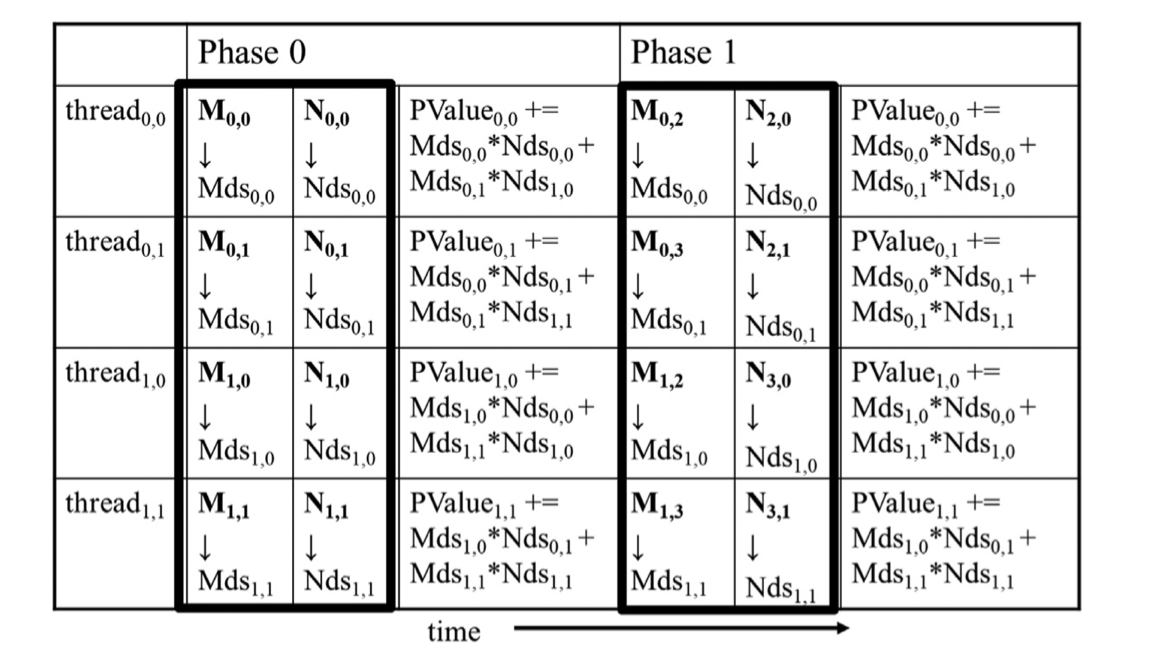
\includegraphics[width=0.9\textwidth]{figs/F5.8.png}
	\caption{\textit{tile矩阵乘法的执行阶段。}}
\end{figure}

请注意,每个点积的计算现在分两个阶段执行,如图 5.8 中的阶段 1 和阶段 2 所示。 
在每个阶段中,每个线程将两对输入矩阵元素的乘积累加到 Pvalue 变量中。 
请注意,Pvalue 是一个自动变量,因此会为每个线程生成一个私有版本。 
我们添加下标只是为了澄清这些是为每个线程创建的 Pvalue 变量的不同实例。 
第一阶段计算如图5.8第四列所示,第二阶段计算如图5.8第七列所示。 
一般来说,如果输入矩阵的维度为 Width 并且tile大小为 TILE\_WIDTH,则点积将在 Width/TILE\_WIDTH 阶段执行。 
这些阶段的创建是减少对全局内存的访问的关键。 每个阶段都专注于输入矩阵值的一个小子集,
线程可以协作地将子集加载到共享内存中,并使用共享内存中的值来满足该阶段中的重叠输入需求。

另请注意,Mds 和 Nds 可以跨阶段重复使用。 
在每个阶段中,相同的 Mds 和 Nds 被重复使用来保存该阶段中使用的 M 和 N 元素的子集。 
这允许更小的共享内存来服务对全局内存的大部分访问。 这是因为每个阶段都专注于输入矩阵元素的一小部分。 
这种集中的访问行为称为局部性。 当算法表现出局部性时,就有机会使用小型高速内存来服务大多数访问,
并将这些访问从全局内存中删除。 
局部性对于在多核 CPU 中实现高性能与在多线程 GPU 中一样重要,我们将在第 6 章“性能注意事项”中回到局部性概念。

\subsection{tile矩阵乘法kernel}
\begin{figure}[H]
	\centering
	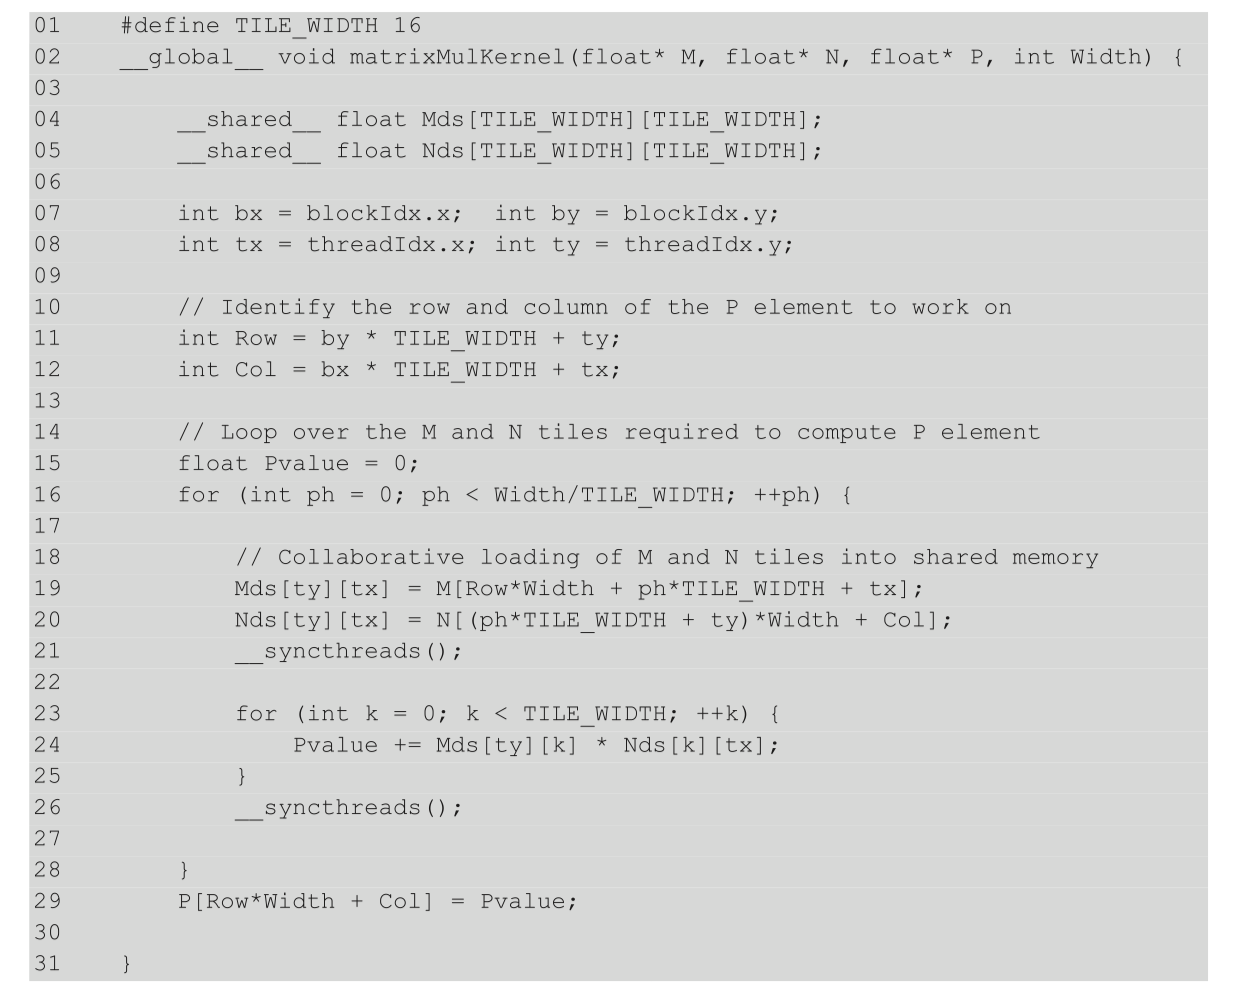
\includegraphics[width=0.9\textwidth]{figs/F5.9.png}
	\caption{\textit{使用共享内存的tile矩阵乘法kernel。}}
\end{figure}

我们现在准备提出一个tile矩阵乘法kernel,它使用共享内存来减少全局内存的流量。 
图 5.9 所示的kernel实现了图 5.8 所示的阶段。 在图 5.9 中,第 04 行和第 05 行分别声明 Mds 和 Nds 为共享内存数组。 
回想一下,共享内存变量的范围是一个block。 因此,将为每个块创建一个版本的 Mds 和 Nds 数组,
并且块的所有线程都可以访问相同的 Mds 和 Nds 版本。 
这很重要,因为块中的所有线程都必须有权访问由其对等方加载到 Mds 和 Nds 中的 M 和 N 元素,
以便它们可以使用这些值来满足其输入需求。

第07行和第08行将threadIdx和blockIdx值保存到名称较短的自动变量中,以使代码更加简洁。 
回想一下,自动标量变量被放入寄存器中。 它们的范围是在每个单独的线程中。 
也就是说,运行时系统为每个线程创建一个私有版本的 tx、ty、bx 和 by,并将驻留在线程可访问的寄存器中。 
它们使用 threadIdx 和 blockIdx 值进行初始化,并在线程的生命周期内多次使用。 一旦线程结束,这些变量的值就不再存在。

第 11 行和第 12 行分别确定线程要生成的 P 元素的行索引和列索引。 该代码假设每个线程负责计算一个 P 元素。 
如第 12 行所示,线程要生成的 P 元素的水平 (x) 位置或列索引可以计算为 bx × TILE\_WIDTH+tx。 
这是因为每个block在水平维度上覆盖了 P 的 TILE\_WIDTH 元素。 
bx block中的线程之前将有 bx 个线程block,或 (bx * TILE\_WIDTH) 个线程; 
它们覆盖 P 的 bx * TILE\_WIDTH 元素。同一块内的另一个 tx 线程将覆盖另一个 tx 元素。 
因此,具有 bx 和 tx 的线程应该负责计算 x 索引为 bx * TILE\_WIDTH+tx 的 P 元素。 
对于图 5.7 中的示例,要由 $block_{1,0}$ 的 $thread_{0,1}$ 计算的 P 元素的水平 (x) 索引为 0 × 2+1=1。 
该水平索引保存在线程的变量 Col 中,如图 5.10 所示。

类似地,要由线程处理的 P 元素的垂直 (y) 位置或行索引的计算方式为 by * TILE\_WIDTH+ty。 
回到图 5.7 中的示例,$block_{1,0}$ 的 $thread_{0,1}$ 计算的 P 元素的 y 索引为 1 × 2+0=2。 
该垂直索引保存在线程的变量 Row 中。  如图5.10所示,每个线程计算Colth列和Rowth行的P元素。 
因此 $block_{1,0}$ 的 $thread_{0,1}$ 要计算的 P 元素是 $P_{2,1}$ 。

图 5.9 的第 16 行标记了循环的开始,该循环迭代计算 P 元素的所有阶段。 
循环的每次迭代对应于图 5.8 所示的计算的一个阶段。 ph 变量表示点积已完成的阶段数。 
回想一下,每个阶段都使用 M 个元素的一个tile和 N 个元素的一个tile。 
因此,在每个阶段开始时,前面的阶段已处理了 M 和 N 个元素的 ph × TILE\_WIDTH 对。

\begin{figure}[H]
	\centering
	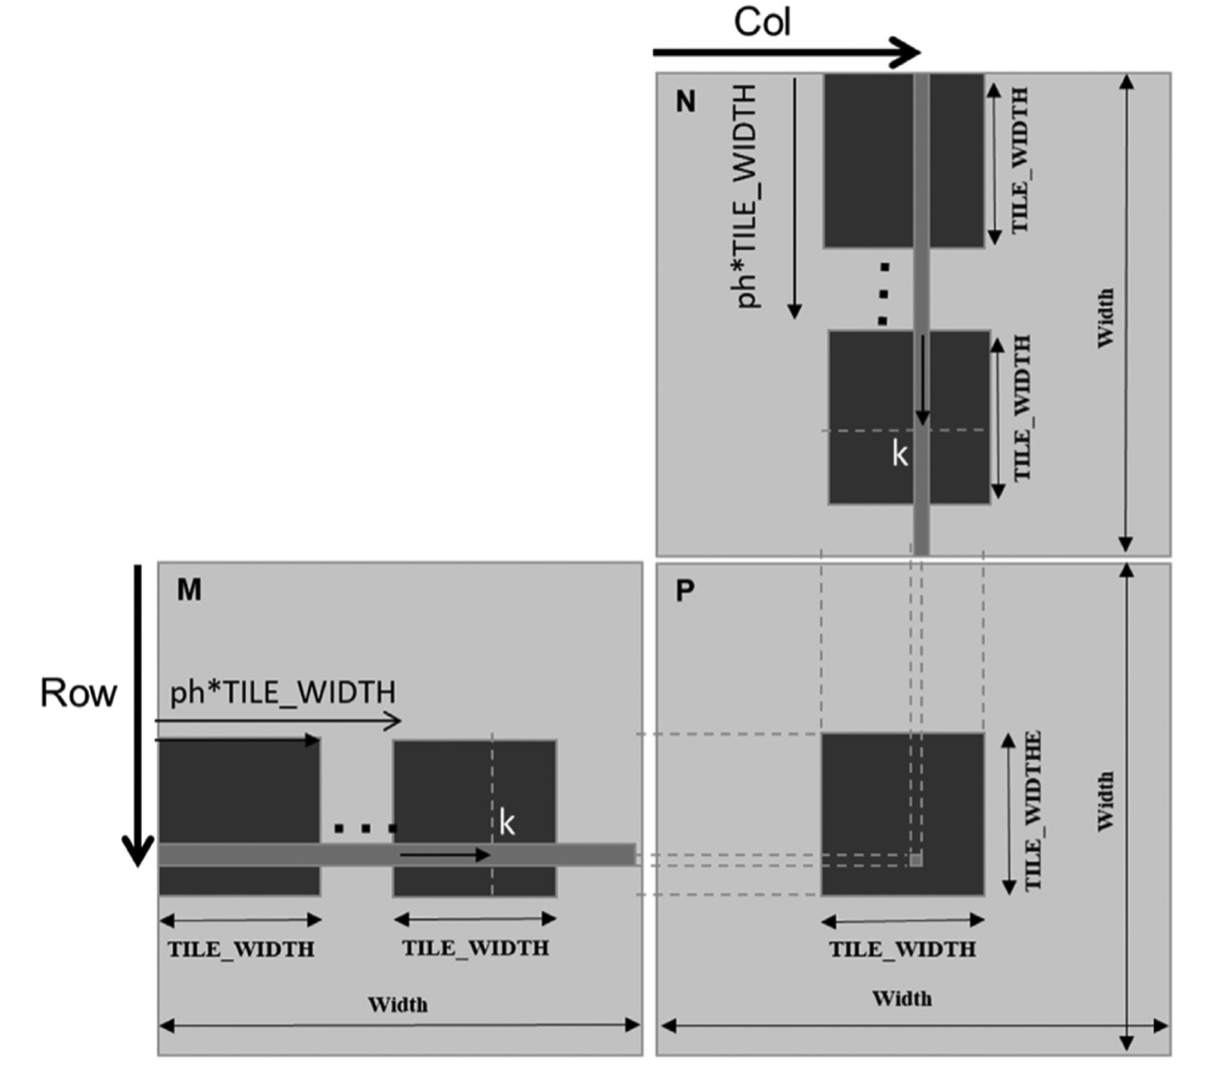
\includegraphics[width=0.9\textwidth]{figs/F5.10.png}
	\caption{\textit{tile乘法中矩阵索引的计算。}}
\end{figure}

在每个阶段,图 5.9 中的第 19 行和第 20 行分别将适当的 M 和 N 元素加载到共享内存中。 
由于我们已经知道线程要处理的 M 行和 N 列,因此我们现在将重点转向 M 的列索引和 N 的行索引。
如图 5.10 所示,每个块有 TILE\_WIDTH$^2$ 个线程, 
将协作将 TILE\_WIDTH$^2$M 元素和 TILE\_WIDTH$^2$N 元素加载到共享内存中。 
因此我们需要做的就是分配每个线程加载一个M元素和一个N元素。 通过使用 blockIdx 和 threadIdx 可以方便地完成此操作。 
请注意,要加载的 M 元素部分的起始列索引是 ph * TILE\_WIDTH。 
因此,一种简单的方法是让每个线程加载一个距离该起始点 tx(threadIdx.x 值)位置的元素。 
同样,要加载的 N 个元素的部分的起始行索引也是 ph * TILE\_WIDTH。 
因此,每个线程都会加载距该起始点 ty(threadIdx.y 值)位置的元素。

这正是第 19 行和第 20 行中的内容。在第 19 行中,
每个线程加载 M[Row * Width + ph * TILE\_WIDTH + tx],
其中线性化索引由行索引 Row 和列索引 ph * TILE\_WIDTH +tx 组成。 
由于 Row 是 ty 的线性函数,每个 TILE\_WIDTH 线程都会将唯一的 M 元素加载到共享内存中,
因为每个线程都有唯一的 tx 和 ty 组合。 这些线程将一起加载图 5.10 中 M 的暗方形子集。 
以类似的方式,在第 20 行中,
每个线程使用线性化索引 (ph × TILE\_WIDTH + ty) × Width + Col 将适当的 N 元素加载到共享内存。
读者应该使用图 1 和 2 中的小示例。 5.7 和 5.8 来验证各个线程的地址计算是否正确。

第 21 行中的barrier \_\_syncthreads() 确保所有线程都已完成将 M 和 N 的tile加载到 Mds 和 Nds 中,然后才能继续前进。 
回想一下第 4 章“计算架构和调度”,对 \_\_syncthreads() 的调用可用于使块中的所有线程相互等待到达barrier,
然后才能继续执行。 这很重要,因为线程使用的 M 和 N 元素可以由其他线程加载。 在任何线程开始使用元素之前,
需要确保所有元素都已正确加载到共享内存中。 然后,第 23 行中的循环基于tile元素执行点积的一阶段。 
线程 ty、tx 的循环流程如图 5.10 所示,其中 M 和 N 元素的访问方向沿箭头标记为 k,即第 23 行的循环变量。
注意,这些元素将从 Mds 访问 Nds,保存这 M 和 N 个元素的共享内存阵列。 
第 26 行中的barrier \_\_syncthreads() 确保所有线程都已完成对共享内存中 M 和 N 元素的使用,
然后再进行下一次迭代并加载下一个tile中的元素。 因此,没有线程会过早加载元素并破坏其他线程的输入值。

第 21 行和第 26 行中的两个 \_\_syncthreads() 调用演示了两种不同类型的数据依赖关系,
并行程序员在线程之间进行协调时通常必须对其进行推理。 第一种称为写后读依赖,
因为线程在尝试读取数据之前必须等待其他线程将数据写入正确的位置。 第二种称为读后写依赖,
因为线程必须等待所有需要该数据的线程读取该数据,然后才能覆盖该数据。 
写后读和读后写依赖性的其他名称分别是真依赖性和假依赖性。 先读后写依赖是真正的依赖,
因为读线程确实需要写线程提供的数据,所以它别无选择,只能等待。 读后写依赖是一种错误依赖,
因为写入线程不需要来自读取线程的任何数据。 这种依赖性是由于它们重复使用相同的内存位置而引起的,
如果它们使用不同的位置,则不会存在这种依赖性。

从第 16 行到第 28 行的循环嵌套说明了一种称为strip-mining的技术,该技术采用长时间运行的循环并将其分成多个阶段。 
每个阶段都涉及一个内部循环,该循环执行原始循环的几次连续迭代。 原始循环成为外循环,其作用是迭代地调用内循环,
以便原始循环的所有迭代都按其原始顺序执行。 通过在内循环之前和之后添加barrier同步,
我们强制同一块中的所有线程在每个阶段将其工作重点放在输入数据的同一部分上。 
strip-mining是创建数据并行程序中tile所需阶段的重要手段
\footnote{读者应该注意到,strip-mining长期以来一直用于 CPU 编程。 
strip-mining后进行循环交换通常用于启用tile以改进顺序程序中的局部性。 
strip-mining也是矢量化编译器为 CPU 程序生成矢量或 SIMD 指令的主要工具。}。

点积的所有阶段完成后,执行退出外循环。 在第 29 行中,所有线程使用根据 Row 和 Col 计算出的线性化索引写入其 P 元素。

tile算法的好处是巨大的。 对于矩阵乘法,全局内存访问减少了 TILE\_WIDTH 倍。 
通过 $16 \times 16$ 个区块,可以将全局内存访问减少 16 倍。这将计算与全局内存访问的比率从 0.25 OP/B 增加到 4 OP/B。 
这一改进使得 CUDA GPU的内存带宽能够支持更高的计算速率。 
例如,在全局内存带宽为 1555 GB/秒的 A100 GPU 中,
这一改进使GPU能够实现 (1555 GB/秒) × (4 OP/B)=6220 GFLOPS,大大高于 389 未使用tile的kernel实现的 GFLOPS。

尽管分块显着提高了吞吐量,但 6220 GFLOPS 仍然仅为GPU峰值吞吐量 19,500 GFLOPS 的 32\%。 
可以进一步优化代码以减少全局内存访问次数并提高吞吐量。 我们将在本书后面看到其中一些优化,而其他高级优化将不会涉及。 
由于矩阵乘法在许多领域中的重要性,因此存在高度优化的库,例如 cuBLAS 和 CUTLASS,它们已经包含了许多高级优化。 
程序员可以使用这些库立即在其线性代数应用程序中实现接近峰值的性能。

tile在提高矩阵乘法吞吐量(特别是一般应用程序)方面的有效性并不是 GPU 所独有的。 
应用tile(或阻塞)技术来提高 CPU 性能的历史由来已久,方法是确保在特定时间窗口内由 CPU 线程重用的数据能够在缓存中找到。 
一个关键的区别是,CPU 上的tile技术依赖 CPU 缓存来隐式地将重用数据保留在on-chip,
而 GPU 上的tile技术显式地使用共享内存来将数据保留在on-chip。 原因是 CPU 核心通常一次运行一两个线程,
因此线程可以依赖缓存来保存最近使用的数据。 相比之下,GPU SM 同时运行多个线程以隐藏延迟。 
这些线程可能会竞争缓存槽,这会降低 GPU 缓存的可靠性,从而需要使用共享内存来存储要重用的重要数据。

虽然tile矩阵乘法kernel的性能改进令人印象深刻,但它确实做了一些简化的假设。 首先,假设矩阵的宽度是线程块宽度的倍数。 
这会阻止kernel正确处理任意宽度的矩阵。 第二个假设是矩阵是方阵。 在实践中情况并不总是如此。 
在下一节中,我们将提出一个带有边界检查的kernel,以消除这些假设。

\subsection{边界检查}
\begin{figure}[H]
	\centering
	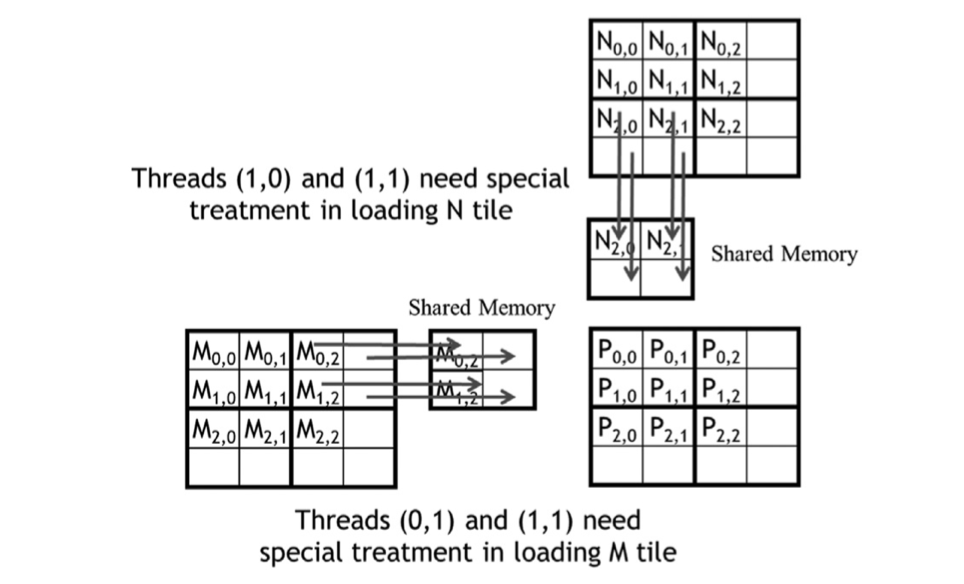
\includegraphics[width=0.9\textwidth]{figs/F5.11.png}
	\caption{\textit{加载靠近边缘的输入矩阵元素:$block_{0,0}$ 的阶段 1。}}
\end{figure}

我们现在扩展tile矩阵乘法kernel来处理任意宽度的矩阵。 扩展必须允许kernel正确处理宽度不是tile宽度倍数的矩阵。 
让我们将图 5.7 中的小示例更改为使用 $3 \times 3$ M、N 和 P 矩阵。 修改后的例子如图5.11所示。 
请注意,矩阵的宽度为 3,它不是tile宽度(2)的倍数。 图 5.11 显示了 $block_{0,0}$ 第二阶段期间的内存访问模式。 
我们看到 $thread_{0,1}$ 和 $thread_{1,1}$ 将尝试加载M个不存在的元素。 
类似地,我们看到 $thread_{1,0}$ 和 $thread_{1,1}$ 将尝试访问N个不存在的元素。

访问不存在的元素有两个问题。 在访问超出行末尾的不存在元素的情况下(图 5.11 中线程 0,1 和线程 1,1 的 M 访问),
这些访问将针对不正确的元素进行。 在我们的示例中,线程将尝试访问不存在的 $M_{0,3}$ 和 $M_{1,3}$ 。 
那么这些内存负载会发生什么情况呢? 要回答这个问题,我们需要回到二维矩阵的线性化布局。 
线性化布局中 $M_{0,2}$ 之后的元素是 $M_{1,0}$ 。 
尽管 $thread_{0,1}$ 尝试访问 $M_{0,3}$ ,但最终会获得 $M_{1,0}$ 。 
在随后的内积计算中使用该值显然会破坏输出值。

访问超出列末尾的元素时也会出现类似的问题(图 5.11 中 $thread_{1,0}$ 和 $thread_{1,1}$ 进行 N 次访问)。 
这些访问是对数组分配区域之外的内存位置的访问。 在某些系统中,它们将从其他数据结构返回随机值。 
在其他系统中,这些访问将被拒绝,导致程序中止。 无论哪种方式,此类访问的结果都是不理想的。

\begin{figure}[H]
	\centering
	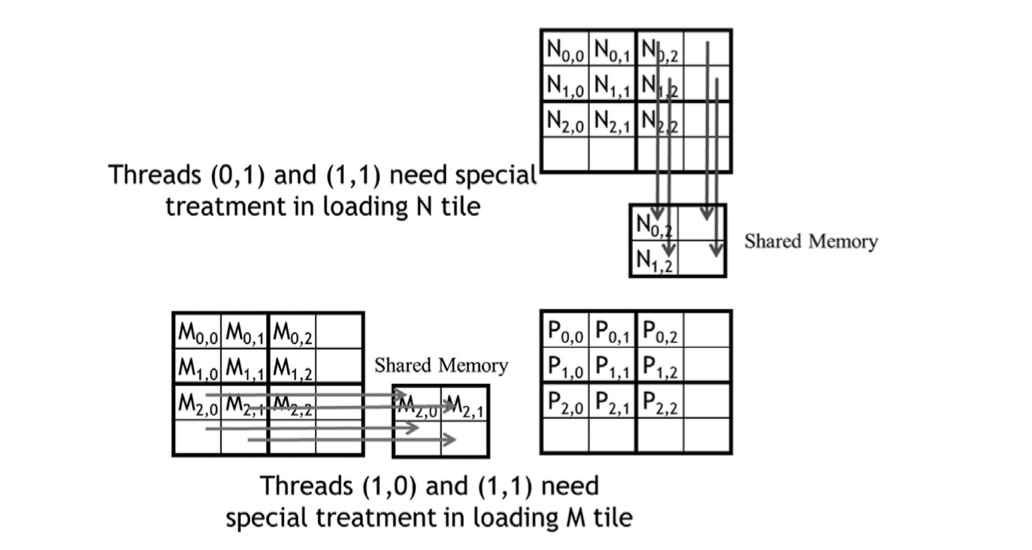
\includegraphics[width=0.9\textwidth]{figs/F5.12.png}
	\caption{\textit{在 $block_{1,1}$ 的阶段 0 期间加载输入元素。}}
\end{figure}

从我们到目前为止的讨论来看,有问题的访问似乎只出现在线程执行的最后阶段。 
这表明我们可以通过在tile kernel执行的最后阶段采取特殊操作来处理它。 不幸的是,事实并非如此。 
有问题的访问可能出现在所有阶段。 图 5.12 显示了阶段 0 期间 $block_{1,1}$ 的内存访问模式。
我们看到 $thread_{1,0}$ 和 $thread_{1,1}$ 尝试访问不存在的 M 元素 $M_{3,0}$ 和 $M_{3,1}$ ,
而 $thread_{0,1}$ 和 $thread_{1,1}$ 尝试访问不存在的 $N_{0,3}$ 和 $N_{1,3}$ 。

请注意,这些有问题的访问不能通过简单地排除不计算有效 P 元素的线程来阻止。 
例如,$block_{1,1}$ 中的 $thread_{1,0}$ 不计算任何有效的 P 元素。 
然而,它需要在阶段0期间加载 $M_{2,1}$ 以供 $block_{1,1}$中的其他线程使用。 
此外,请注意,某些计算有效 P 元素的线程将尝试访问不存在的 M 或 N 元素。 
例如,如图 5.11 所示,$block_{0,0}$ 的 $thread_{0,1}$ 计算有效的 P 元素 $P_{0,1}$ 。 
然而,它在阶段 1 期间尝试访问不存在的 $M_{0,3}$。这两个事实表明我们需要使用不同的边界条件测试来加载 M 个tile、
加载 N 个tile以及计算/存储 P 元素。 要遵循的经验法则是,每次内存访问都需要进行相应的检查,
以确保访问中使用的索引位于正在访问的数组的范围内。

让我们从加载输入tile的边界测试条件开始。 当线程要加载输入tile元素时,它应该测试它尝试加载的输入元素是否是有效元素。 
通过检查 y 和 x 索引可以轻松完成此操作。 例如,在图 5.9 中的第 19 行中,
线性化索引是从 Row 的 y 索引和 ph × TILE\_WIDTH + tx 的 x 索引导出的。 
边界条件测试是两个索引均小于宽度: Row < Width \&\& (ph * TILE\_WIDTH+tx) < Width。 
如果条件为真,线程应该继续加载 M 元素。 
读者应该验证加载 N 元素的条件测试是 (ph * TILE\_WIDTH +ty) < Width \&\& Col < Width 。

如果条件为 false,则线程不应加载该元素。 问题是应该将什么放入共享内存位置。 
答案是0.0,这个值在内积计算中使用不会造成任何危害。 如果任何线程在计算其内积时使用这个0.0值,则内积值不会有任何变化。

最后,只有当线程负责计算有效的 P 元素时,才应存储其最终内积值。 
此条件的测试是 (Row < Width) \&\& (Col < Width)。 具有附加边界条件检查的kernel代码如图 5.13 所示。

\begin{figure}[H]
	\centering
	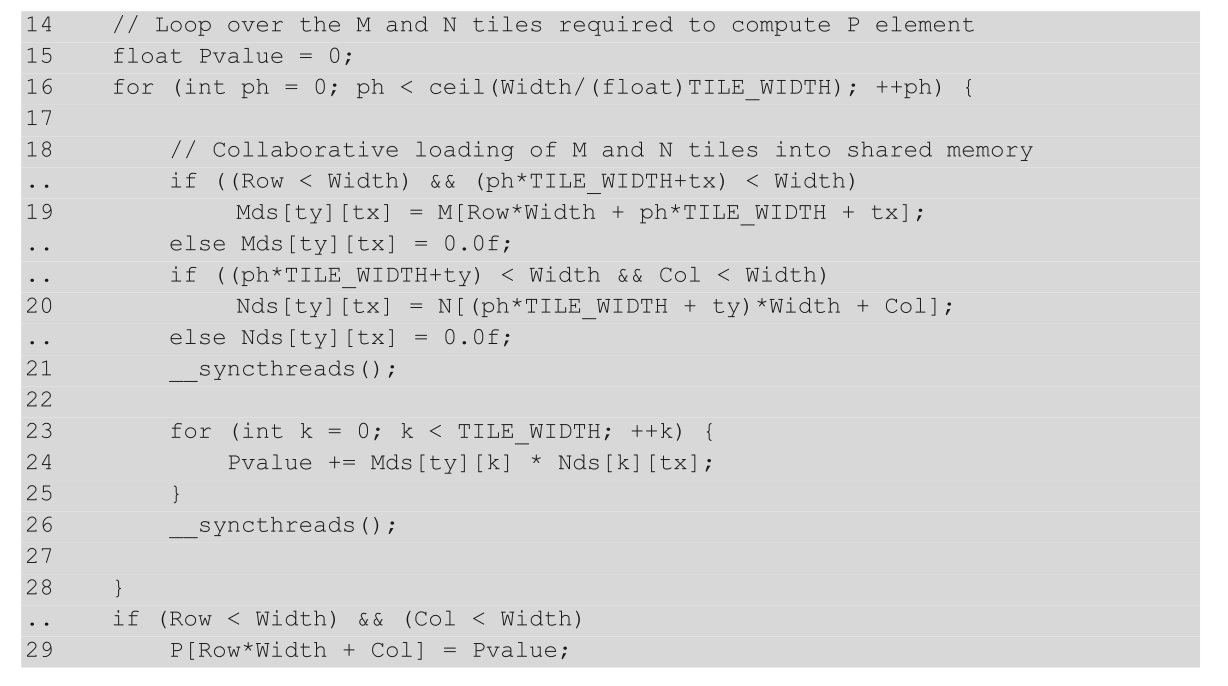
\includegraphics[width=0.9\textwidth]{figs/F5.13.png}
	\caption{\textit{具有边界条件检查的tile矩阵乘法kernel。}}
\end{figure}

通过边界条件检查,tile矩阵乘法kernel距离通用矩阵乘法kernel仅一步之遥。 
一般来说,矩阵乘法是针对矩形矩阵定义的:j x k M 矩阵与 k x l N 矩阵相乘会得到 j x l P 矩阵。 
到目前为止,我们的kernel只能处理方阵。

幸运的是,将我们的kernel进一步扩展为通用矩阵乘法kernel非常容易。 我们需要做一些简单的改变。 
首先,宽度参数被三个无符号整数参数替换:j、k、l。 其中Width用于指M的高度或P的高度,将其替换为j。 
其中Width用于指M的宽度或N的高度,将其替换为k。 其中Width用于指N的宽度或P的宽度,将其替换为l。 
对kernel进行这些更改的修订留作练习。

\subsection{内存使用对占用的影响}
回想一下,在第 4 章“计算架构和调度”中,我们讨论了最大化 SM 上线程的占用率以能够容忍长延迟操作的重要性。 
kernel的内存使用情况在占用调整中起着重要作用。 虽然 CUDA 寄存器和共享内存可以非常有效地减少对全局内存的访问次数,
但必须小心保持在这些内存的 SM 容量范围内。 每个 CUDA GPU提供的资源有限,
这限制了给定应用程序可以同时驻留在 SM 中的线程数量。 一般来说,每个线程需要的资源越多,每个SM中可以驻留的线程数量就越少。

我们在第 4 章“计算架构和调度”中看到,寄存器的使用如何成为占用的限制因素。 
共享内存的使用还可以限制可以分配给每个 SM 的线程数量。 例如,A100 GPU 可配置为每个 SM 最多具有 164 KB 共享内存,
并且每个 SM 最多支持 2048 个线程。 因此,对于要使用的所有 2048 个线程槽,
线程块使用的平均值不应超过 (164 KB)/(2048 个线程)=82 B/线程。 在tile矩阵乘法示例中,
每个块都有 2 个 TILE\_WIDTH 线程,并为 Mds 使用 TILE\_WIDTH$^2$ × 4B 共享内存,
为 Nds 使用 TILE\_WIDTH$^2$ × 4B 共享内存。 
因此,线程块平均使用 (TILE\_WIDTH$^2$ × 4B + TILE\_WIDTH$^2$ × 4B)/(TILE\_WIDTH$^2$ 个线程)=8 B/线程共享内存。 
因此,tile矩阵乘法kernel的占用不受共享内存的限制。

但是,请考虑一个具有使用 32 KB 共享内存的线程块的kernel,每个线程块有 256 个线程。 
在这种情况下,kernel平均使用 (32 KB)/(256 个线程)=132 B/线程的共享内存。 
在这样的共享内存使用情况下,kernel无法实现完全占用。 每个 SM 最多只能托管 (164 KB)/(132 B/线程)=1272 个线程。 
因此,该kernel可达到的最大占用率为(1272 个分配的线程)/(2048 个最大线程)=62\%。

请注意,每个 SM 中的共享内存大小也可能因GPU而异。 每一代或每一型号的GPU在每个 SM 中可以具有不同数量的共享内存。 
通常希望kernel能够根据硬件中的可用量使用不同数量的共享内存。 
也就是说,我们可能希望CPU代码动态确定共享内存的大小并调整kernel使用的共享内存量。 
这可以通过调用 cudaGetDeviceProperties 函数来完成。 假设变量 \&devProp 被传递给函数。 
在本例中,字段 devProp。 sharedMemPerBlock 给出每个 SM 中可用的共享内存量。 
然后,程序员可以确定每个块应使用的共享内存量。

不幸的是,图中的kernel。 5.9 和 5.13 不支持CPU代码对共享内存使用情况的任何动态调整。 
图 5.9 中使用的声明将其共享内存使用量的大小硬连接到编译时常量:

\_\_shared\_\_ float Mds[TILE\_WIDTH][TILE\_WIDTH];
\_\_shared\_\_ float Nds[TILE\_WIDTH][TILE\_WIDTH];

也就是说,无论编译时 TILE\_WIDTH 的值设置为多少,Mds 和 Nds 的大小都设置为 TILE\_WIDTH 2 个元素。 由于代码包含

\#define TILE\_WIDTH 16

Mds 和 Nds 都有 256 个元素。 如果我们想改变Mds和Nds的大小,我们需要改变TILE\_WIDTH的值并重新编译代码。 
如果不重新编译,kernel无法在运行时轻松调整其共享内存使用情况。

我们可以通过在共享内存声明前面添加 C extern 关键字并在声明中省略数组的大小,
在 CUDA 中使用不同风格的声明来启用此类调整。 基于这种风格,Mds 和 Nds 的声明需要合并到一个动态分配的数组中:

extern \_\_shared\_\_ Mds\_Nds[];

由于只有一个合并数组,因此我们还需要手动定义数组的 Mds 部分的起始位置和 Nds 部分的起始位置。 
请注意,合并后的数组是一维的。 我们需要使用基于垂直和水平索引的线性化索引来访问它。

在运行时,当我们调用kernel时,我们可以根据GPU查询结果动态配置每个块要使用的共享内存量,
并将其作为第三个配置参数提供给kernel调用。 例如,可以使用以下语句启动修订后的kernel:

\begin{figure}[H]
	\centering
	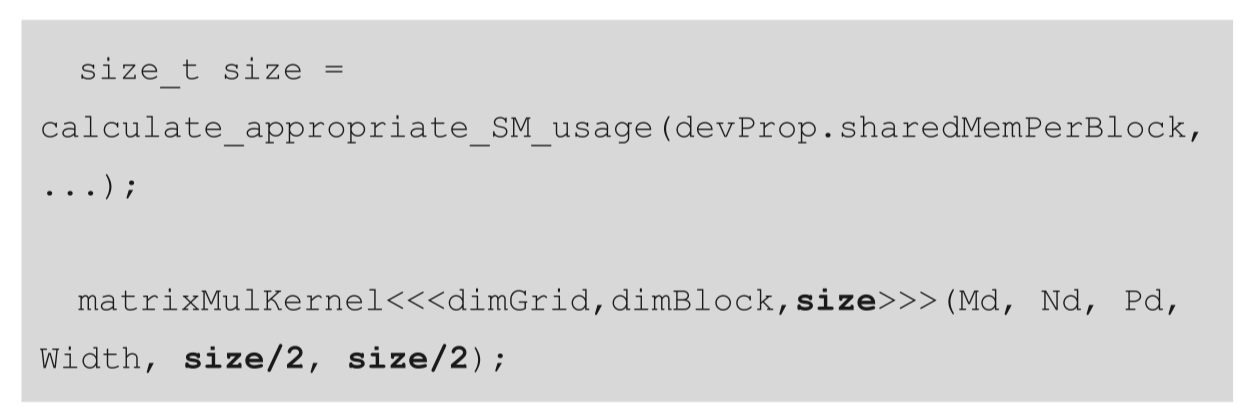
\includegraphics[width=0.9\textwidth]{figs/F5-a.2.png}
\end{figure}

其中 size\_t 是一个内置类型,用于声明一个变量来保存动态分配的数据结构的大小信息。 
大小以字节数表示。 在我们的矩阵乘法示例中,对于 16 x 16 块,我们的大小为 2 x 16 x 16 x 4=2048 字节,
以容纳 Mds 和 Nds。 我们省略了运行时设置 size 值的计算细节,并将其作为读者的练习。

在图 5.14 中,我们展示了如何修改图 5.14 和 5.14 中的kernel代码。 
5.9 和 5.11 为 Mds 和 Nds 数组使用动态大小的共享内存。 将数组每个部分的大小作为参数传递到kernel函数中也可能很有用。 
在此示例中,我们添加了两个参数:第一个参数是 Mds 部分的大小,第二个参数是 Nds 部分的大小,均以字节为单位。 
请注意,在上面的CPU代码中,我们传递了 size/2 作为这些参数的值,即 1024 字节。 通过第 06 行和第 07 行的赋值,
kernel代码的其余部分可以使用 Mds 和 Nds 作为数组的基数,并使用线性化索引来访问 Mds 和 Nds 元素。 
例如,不使用 Mds[ty][tx],而是使用 Mds[ty * TILE\_WIDTH+tx]。

\begin{figure}[H]
	\centering
	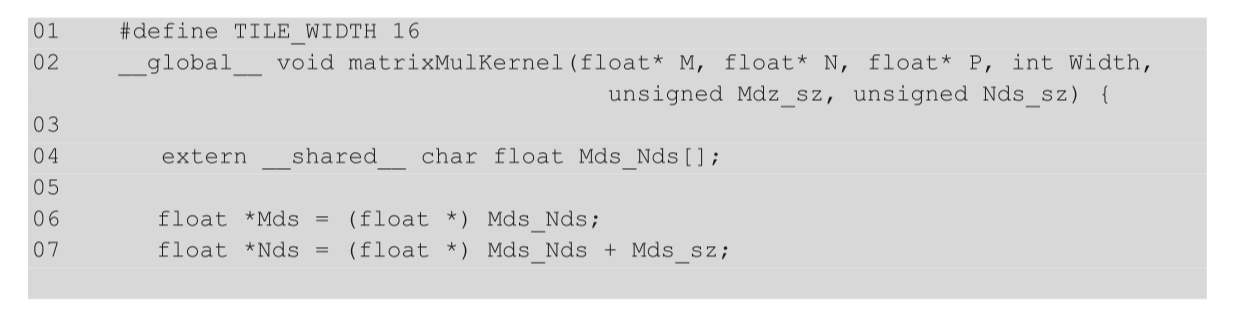
\includegraphics[width=0.9\textwidth]{figs/F5.14.png}
	\caption{\textit{具有动态大小共享内存使用量的tile矩阵乘法kernel。}}
\end{figure}

\subsection{总结}
总之,现代处理器中程序的执行速度可能受到内存速度的严重限制。 为了充分利用 CUDA GPU的执行吞吐量,
需要在kernel代码中争取较高的计算与全局内存访问比率。 如果该比率较低,则kernel受内存限制。 
也就是说,它的执行速度受到从内存访问其操作数的速率的限制。

CUDA 提供对寄存器、共享内存和常量内存的访问。 这些内存比全局内存小得多,但可以以更高的速度访问。 
有效地使用这些内存需要重新设计算法。 我们以矩阵乘法为例来说明tile,
这是一种增强数据访问局部性并有效利用共享内存的流行策略。 
在并行编程中,tile使用barrier同步来强制多个线程在执行的每个阶段共同关注输入数据的子集,
以便可以将子集数据放入这些特殊的内存类型中,从而实现更高的访问速度。

然而,对于 CUDA 程序员来说,了解这些特殊类型内存的有限大小非常重要。 他们的能力取决于实施。 
一旦超出其容量,它们就会限制每个 SM 中可以同时执行的线程数量,并可能对 GPU 的计算吞吐量及其容忍延迟的能力产生负面影响。 
开发应用程序时推理硬件限制的能力是并行编程的一个关键方面。

尽管我们在 CUDA C 编程环境中引入了tile算法,但它是在几乎所有类型的并行计算系统中实现高性能的有效策略。 
原因是应用程序必须在数据访问中表现出局部性,才能有效利用这些系统中的高速内存。 
例如,在多核CPU系统中,数据局部性允许应用程序有效地使用on-chip数据缓存来减少内存访问延迟并实现高性能。 
这些on-chip数据缓存的大小也有限,并且要求计算表现出局部性。 
因此,读者也会发现在使用其他编程模型为其他类型的并行计算系统开发并行应用程序时,tile算法很有用。

本章的目标是介绍局部性、tile和不同 CUDA 内存类型的概念。 我们引入了使用共享内存的tile矩阵乘法kernel。 
我们进一步研究了边界测试条件的需求,以在应用tile技术时允许任意数据维度。 
我们还简要讨论了动态大小共享内存分配的使用,以便kernel可以根据硬件能力调整每个块使用的共享内存的大小。 
我们没有讨论寄存器在tile中的使用。 当我们在本书的第二部分讨论并行算法模式时,我们将解释寄存器在tile算法中的使用。
